% Latex template: mahmoud.s.fahmy@students.kasralainy.edu.eg
% For more details: https://www.sharelatex.com/learn/Beamer

\documentclass[aspectratio=1610]{beamer}					% Document class

\setbeamertemplate{footline}[text line]{%
  \parbox{\linewidth}{\vspace*{-8pt}Bell's Inequality \hfill\insertshortauthor\hfill\insertpagenumber}}
\setbeamertemplate{navigation symbols}{}

\usepackage[english]{babel}				% Set language
\usepackage[utf8x]{inputenc}			% Set encoding

\mode<presentation>						% Set options
{
  \usetheme{default}					% Set theme
  \usecolortheme{default} 				% Set colors
  \usefonttheme{default}  				% Set font theme
  \setbeamertemplate{caption}[numbered]	% Set caption to be numbered
}

% Uncomment this to have the outline at the beginning of each section highlighted.
%\AtBeginSection[]
%{
%  \begin{frame}{Outline}
%    \tableofcontents[currentsection]
%  \end{frame}
\usepackage{graphicx}					% For including figures
\usepackage{booktabs}					% For table rules
\usepackage{hyperref}	
\usepackage{tikz-network}				% For cross-referencing
\usepackage[absolute,overlay]{textpos}
\usepackage{bm}
\usepackage[font=small,labelfont=bf]{caption}				% For cross-referencing
\usepackage{physics}

\title{Bell's Inequality}	% Presentation title
\author{Clayton W. Seitz}								% Presentation author
\date{\today}									% Today's date	

\begin{document}

% Title page
% This page includes the informations defined earlier including title, author/s, affiliation/s and the date
\begin{frame}
  \titlepage
\end{frame}

\begin{frame}{CHSH and Tsirelson's Inequalities}

\vspace{0.2in}

Alice: $Q,R$
Bob: $S, T$

\vspace{0.1in}
Classical observables distributed according to $P(Q,R,S,T)$. Combination of correlations between Alice and Bobs measurements are bounded according to the CHSH inequality

\begin{align*}
|E(QS) + E(RS) + E(RT) - E(QT)| \leq 2
\end{align*}

For the quantum version, define 4 spin operators along arbitrary directions $Q = \vec{q}\cdot\sigma, R = \vec{r}\cdot\sigma, S = \vec{s}\cdot\sigma, T = \vec{t}\cdot\sigma$.

The book uses $\vec{q} = (0,0,1), \vec{r} = (1,0,0), \vec{s} = (-\frac{1}{\sqrt{2}},0,-\frac{1}{\sqrt{2}}), \vec{t} = (-\frac{1}{\sqrt{2}},0,\frac{1}{\sqrt{2}})$

\begin{align*}
|\langle Q\otimes S\rangle + \langle R\otimes S\rangle  + \langle R\otimes T\rangle  - \langle Q\otimes T\rangle|  \leq 2\sqrt{2}
\end{align*}



\end{frame}

\begin{frame}{Assumptions and objectives}
As in the book, 
Assume $\vec{q},\vec{r}$ and $\vec{s},\vec{t}$ are orthogonal and all $\vec{q},\vec{r},\vec{s},\vec{t}$ live in a plane (say x-z)\\
\vspace{0.2in}
Now draw a set of pure states $\ket{\psi}$ possibly with different degrees of entanglement\\
\vspace{0.2in}
Question:  How does the Tsirelson bound vary across states with different degrees of entanglement?
\end{frame}

\begin{frame}{The Tsirelson bound}

Solution to Problem 2.3 in the book:

\begin{align*}
(Q\otimes S + R\otimes S  + R\otimes T  - Q\otimes T)^{2} = 4I + [Q,R]\otimes [S,T]
\end{align*}
Jensen's inequality:
\begin{align*}
\langle(Q\otimes S + R\otimes S  + R\otimes T  - Q\otimes T)\rangle^{2} &\leq \langle(Q\otimes S + R\otimes S  + R\otimes T  - Q\otimes T)^{2}\rangle \\
&= \langle 4I + [Q,R]\otimes [S,T]\rangle \\
&= 4 + \langle [Q,R]\otimes [S,T]\rangle
\end{align*}

for fixed $Q,R,S,T$.

\end{frame}

\begin{frame}{The Tsirelson bound}

Using that $(\sigma\cdot \vec{a})(\sigma\cdot \vec{b}) = \vec{a}\cdot \vec{b} + i\sigma\cdot(\vec{a}\times \vec{b})$

\begin{equation*}
[A,B] = i\sigma\cdot(\vec{a}\times\vec{b} - \vec{b}\times\vec{a}) = 2i\sigma\cdot(\vec{a}\times\vec{b})
\end{equation*}

Let $\vec{n} = \vec{q}\times\vec{r}$ and $\vec{m} = \vec{s}\times\vec{t}$. Per our constraints, we could have $\vec{n} = \vec{m} = \hat{y}$.

\begin{align*}
\langle [Q,R]\otimes [S,T]\rangle &= -4\bra{\psi}\sigma\cdot\vec{n}\otimes\sigma\cdot\vec{m}\ket{\psi}\\
&= -4\bra{\psi}\sigma\cdot\hat{y}\otimes\sigma\cdot\hat{y}\ket{\psi}\\
&= -4\bra{\psi}\sigma_{1y}\otimes\sigma_{2y}\ket{\psi}
\end{align*}

\begin{align*}
\langle(Q\otimes S + R\otimes S  + R\otimes T  - Q\otimes T)\rangle \leq 2\sqrt{1-\bra{\psi}\sigma_{1y}\otimes\sigma_{2y}\ket{\psi}}
\end{align*}

\end{frame}

\begin{frame}{Quantifying entanglement: partial traces}

\begin{align*}
\mathrm{Tr}_{A}(\rho_{AB}) &= \sum_{ijkl} \rho_{ij}^{kl} \mathrm{Tr}_{A}(\ket{i}\bra{k}) \otimes \ket{j}\bra{l}\\
&= \sum_{i} \left(\sum_{jl} \rho_{ij}^{il} \ket{j}\bra{l}\right)\\
&= (\rho_{00}^{00}+\rho_{10}^{10})\ket{0}\bra{0} + (\rho_{00}^{01}+\rho_{10}^{11})\ket{0}\bra{1} + (\rho_{01}^{00}+\rho_{11}^{10})\ket{1}\bra{0} + (\rho_{01}^{01}+\rho_{11}^{11})\ket{1}\bra{1}
\end{align*}

\begin{align*}
\mathrm{Tr}_{B}(\rho_{AB}) &= \sum_{ijkl} \rho_{ij}^{kl} \ket{i}\bra{k} \otimes \mathrm{Tr}_{B}(\ket{j}\bra{l})\\
&= \sum_{j} \left(\sum_{ik} \rho_{ij}^{kj} \ket{i}\bra{k}\right)\\
&= (\rho_{00}^{00}+\rho_{01}^{01})\ket{0}\bra{0} + (\rho_{00}^{10}+\rho_{01}^{11})\ket{0}\bra{1} + (\rho_{10}^{00}+\rho_{11}^{01})\ket{1}\bra{0} + (\rho_{10}^{10}+\rho_{11}^{11})\ket{1}\bra{1}
\end{align*}

\end{frame}

\begin{frame}{Reduced density matrices for an arbitrary state}

\begin{align*}
\mathrm{Tr}_{A}(\rho_{AB}) &=
\begin{pmatrix}
\rho_{00}^{00}+\rho_{10}^{10} & \rho_{00}^{01}+\rho_{10}^{11}\\
\rho_{01}^{00}+\rho_{11}^{10} & \rho_{01}^{01}+\rho_{11}^{11}
\end{pmatrix}
= \begin{pmatrix}
|\alpha|^{2} + |\gamma|^{2} & \alpha\beta^{*} + \gamma\delta^{*}\\
\beta\alpha^{*} + \delta\gamma^{*} & |\beta|^{2} + |\delta|^{2}
\end{pmatrix}
\end{align*}

\begin{align*}
\mathrm{Tr}_{B}(\rho_{AB}) &=
\begin{pmatrix}
\rho_{00}^{00}+\rho_{01}^{01} & \rho_{00}^{10}+\rho_{01}^{11}\\
\rho_{10}^{00}+\rho_{11}^{01} & \rho_{10}^{10}+\rho_{11}^{11}
\end{pmatrix}
= \begin{pmatrix}
|\alpha|^{2} + |\beta|^{2} & \alpha\gamma^{*} + \beta\delta^{*}\\
\gamma\alpha^{*} + \delta\beta^{*} & |\gamma|^{2} + |\delta|^{2}
\end{pmatrix}
\end{align*}

\end{frame}

\begin{frame}{Definition of entanglement entropy}

The entanglement entropy of a bipartite system is the Von Neumann entropy of either reduced density matrix (it doesn't matter which one we choose)

\begin{align*}
S(\rho_{A}) = -\mathrm{Tr}(\rho_{A}\log\rho_{A}) = -\sum_{x}\lambda_{x}\log\lambda_{x}
\end{align*}

for eigenvalues $\lambda_{x}$ of $\rho_{A}$. This tells us: do the reduced states $\rho_{A}$ and $\rho_{B}$ contain all the \emph{information} in $\rho_{AB}$?

\end{frame}

\begin{frame}{Entanglement entropy and Tsirelson's bound}

Sanity check:\\
\vspace{0.2in}
Draw random reals $a,b,c,d,e,f,g,h\sim U([0,1]^{8})$\\
\vspace{0.2in}
Construct $\ket{\psi} = (a+ib)\ket{00} + (c+id)\ket{01} + (e+if)\ket{10} + (g+ih)\ket{11}$\\
\vspace{0.2in}
Normalize $\ket{\psi} \rightarrow \frac{\ket{\psi}}{\sum_{n}|c_{n}|^{2}}$\\
\vspace{0.2in}
Compute $S(\rho_{A})$ and $2\sqrt{1-\bra{\psi}\sigma_{1y}\otimes\sigma_{2y}\ket{\psi}}$
\end{frame}

\begin{frame}{Entanglement entropy and Tsirelson's bound}

\begin{figure}
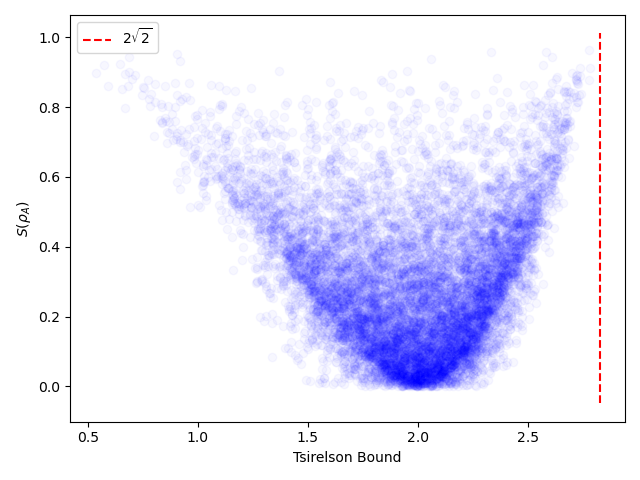
\includegraphics[scale=0.65]{bell.png}
\end{figure}

\end{frame}




\end{document}